%Einleitungstext zum Modul
\section{Klassen}
\graphicspath{{./img/io/}}
Alle Klassen, die für die Funktionen benötigt werden, ohne spezifische Implementierungen zu nennen.
%Bild der Klasse aus dem Klassendiagramm (nur die Klasse jeweils)
%Dokumentation zur Klasse, öffentlichen Methoden und Konstruktor sowie:
%Signal und Slots als Methoden mit Rückgabewert Sigal bzw Slot (zur kenntlichkeit) 
\subsection{InputDataSet}\label{IO:InputDataSet}
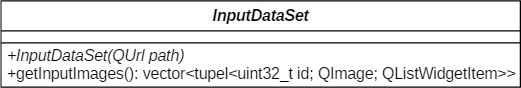
\includegraphics[scale=1, resolution=100]{InputDataSet}\\
Stellt Bilder aus einem Ordner für den Workflow als Eingabedaten bereit. 
\beginMembers
\newMemberAbstract{{InputDataSet}}{QUrl path}{void}{Ist der Konstruktor der Klasse. Lädt alle Bilder die aus "path", versieht diese mit einer Id und generiert zu jedem Bild ein Thumbnail.}
\newMemberAbstract{{getInputImages}}{void}{vector<tuple<uint32\_t, QImage, QListWidgetItem>>}{Gibt die vom Konstruktor erzeugten Daten als Tripel zurück. Die erste Komponente ist die Id, die zweite ein Bild in originaler Auflösung und die dritte ein Objekt vom Typ QListWidgetItem. Darin enthalten ist ein Thumbnail des Bildes welches auf der GUI durch ein QListWidget angezeigt werden kann.}
\closeMembers

\subsection{ResultContext}\label{IO:ResultContext}
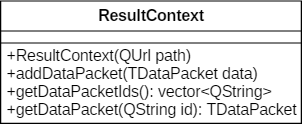
\includegraphics[scale=1, resolution=100]{ResultContext}\\
Erzeugt und repräsentiert den Ergebniskontext auf der Festplatte. Der dabei erzeugte Ordner wird an dem in den Einstellungen definierten Pfad gespeichert. In dem Ordner werden folgende Dateien und Ordner angelegt:
\begin{itemize}
\item globale Einstellungen
\item Einstellungen des Workflows
\item Einstellungen der Algorithmen
\item Log Datei
\item Ergebnisse in je einem Ordner pro Datentyp
\end{itemize}
Die Ids im folgenden korrespondieren mit der in \hyperref[Workflow:IDataPacket]{IDataPacket} definierten Id.
\beginMembers
\newMemberAbstract{{ResultContext}}{QUrl path}{void}{Ist der Konstruktor der Klasse. Erstellt den ResultContext aus vorangegangenen Ergenissen welche im Ordner "path" liegen. }
\newMemberAbstract{{addDataPacket}}{\hyperref[Workflow:TDataPacket]{TDataPacket} data}{void}{Das übergebene Datenpaket wird serialisiert und entsprechend seines \hyperref[Workflow:EDataType]{EDataType} in den Ergebnisordner geschrieben. Benannt wird die Datei nach ihrer Id.}
%todo Darauf hinweisen das Bilder in einem extra Ordner pro DataPacket abgelegt werden.
\newMemberAbstract{{getDataPacketIDs}}{void}{vector<QString>}{Liefert eine Liste mit Ids von allen im Ergebnisordner gefundenen Dateien zurück.}
\newMemberAbstract{{getDataPacket}}{QString id}{\hyperref[Workflow:TDataPacket]{TDataPacket}}{Deserielisiert die Datei mit der Id "id" und gib das Ergebnis als \hyperref[Workflow:TDataPacket]{TDataPacket} zurück.}
\closeMembers

\subsection{ImageIo}\label{IO:ImageIo}
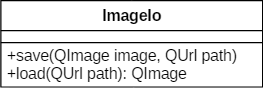
\includegraphics[scale=1, resolution=100]{ImageIO}\\
Stellt die Möglichkeit bereit Bilder zu speichern und zu laden.
\beginMembers
\newMemberAbstract{{save}}{QImage image, QUrl path}{void}{Speichert ein QImage im png-Format an dem in path spezifizierten Ort.}
\newMemberAbstract{{load}}{QUrl path}{QImage}{Lädt ein Bild aus dem in path spezifizierten Ort.}
\closeMembers

\subsection{TextIo}\label{IO:TextIo}
\includegraphics[scale=1, resolution=100]{TextIo}\\
Stellt die Möglichkeit bereit Texte zu speichern und zu laden.
\beginMembers
\newMemberAbstract{{save}}{QUrl path, QString text}{void}{Speichert einen Text in einer in path spezifizierten Datei.}
\newMemberAbstract{{load}}{QUrl path}{QString}{Lädt den Text aus einer in path spezifizierten Datei.}
\closeMembers

\section{Pakete}
Alle genannten Klassen liegen im Paket IO.
%....
\section{Entwurfsmuster}
<Lazy Loading>
Die Klasse \hyperref[IO:ResultContext]{ResultContext} nutzt das Entwurfsmuster Lazy Loading. Sie stellt eine die Liste aller gefundenen Daten zunächst nur als Liste von Ids zur Verfügung. Die einzelnen Datenpakete werden allerdings erst geladen wenn es zu einer konkreten Anfrage kommt.
% verwendete Entwurfsmuster aufzählen erklären etc mit verinfachtem Diagramm (Klassen ohne Inhalt nur die Namen)

\section{Klassendiagramm}
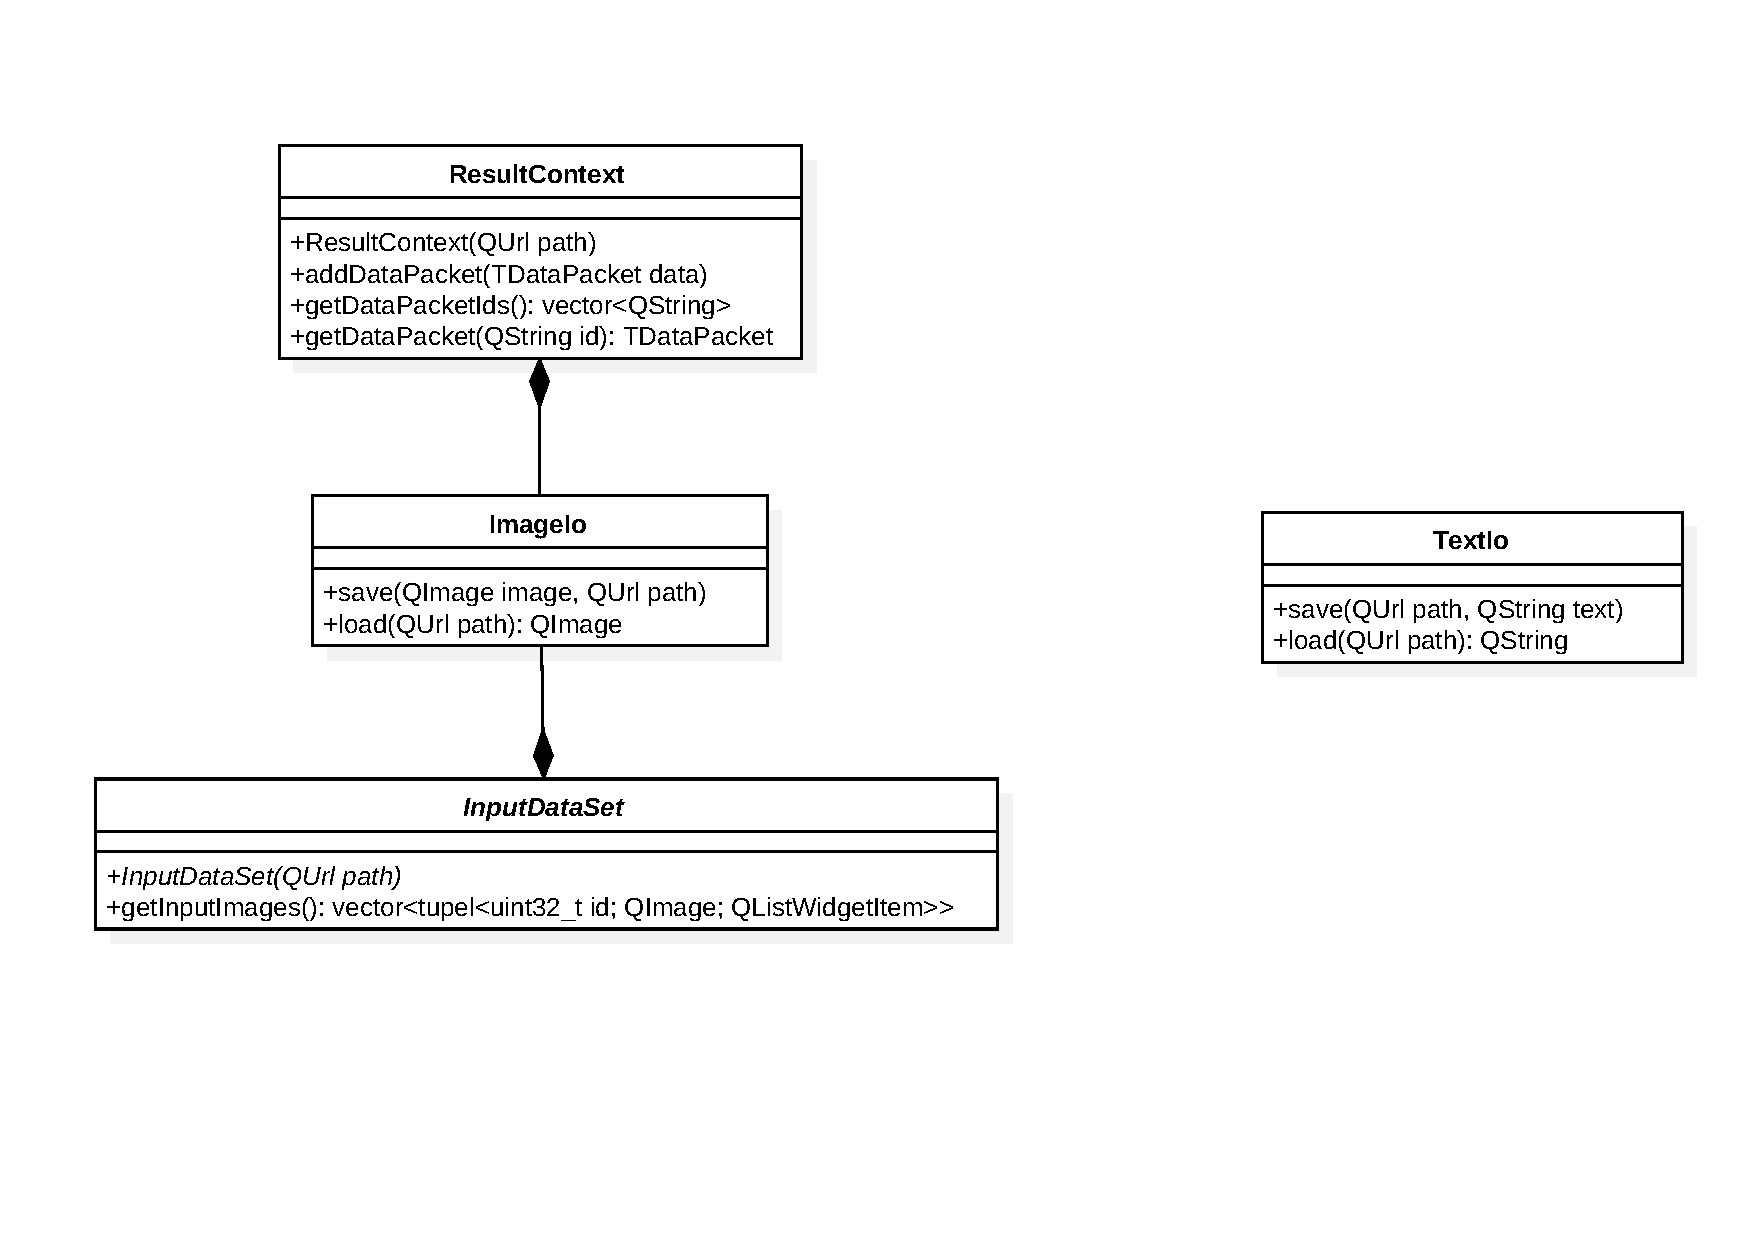
\includegraphics[width=\linewidth]{IoKlassendiagramm.pdf}
%Bitte jeweils kleine Einleitungstexte usw in Unterkapitel gerne auch in Textform Erklärungen zufügen und auf mögliche erweiterungen durch die kann Kriterien eingehen soweit nötig !